\chapter{Model Data} \label{a:data}
This section introduces the data used in the statistical learning model. 

%----------------------------------------------------------------------------------------------------------------------------------------------------------------------------------------------------------
\section*{Study Area}
This study used the monthly unimpaired flows dataset developed and maintained by the California Data Exchange Center (CDEC). The data spans 67 California basins (See Figures \ref{fig:map} and \ref{fig:newtorkmap}) from 1982 to 2014. It can be downloaded with a simple webscraping script available on GitHub. It has approximately 19,000 monthly streamflow observations in acre-feet (AF) and as a continuous variable can be used for regression type studies (See Figure \ref{fig:flows}). 

\begin{figure}
	\centering
	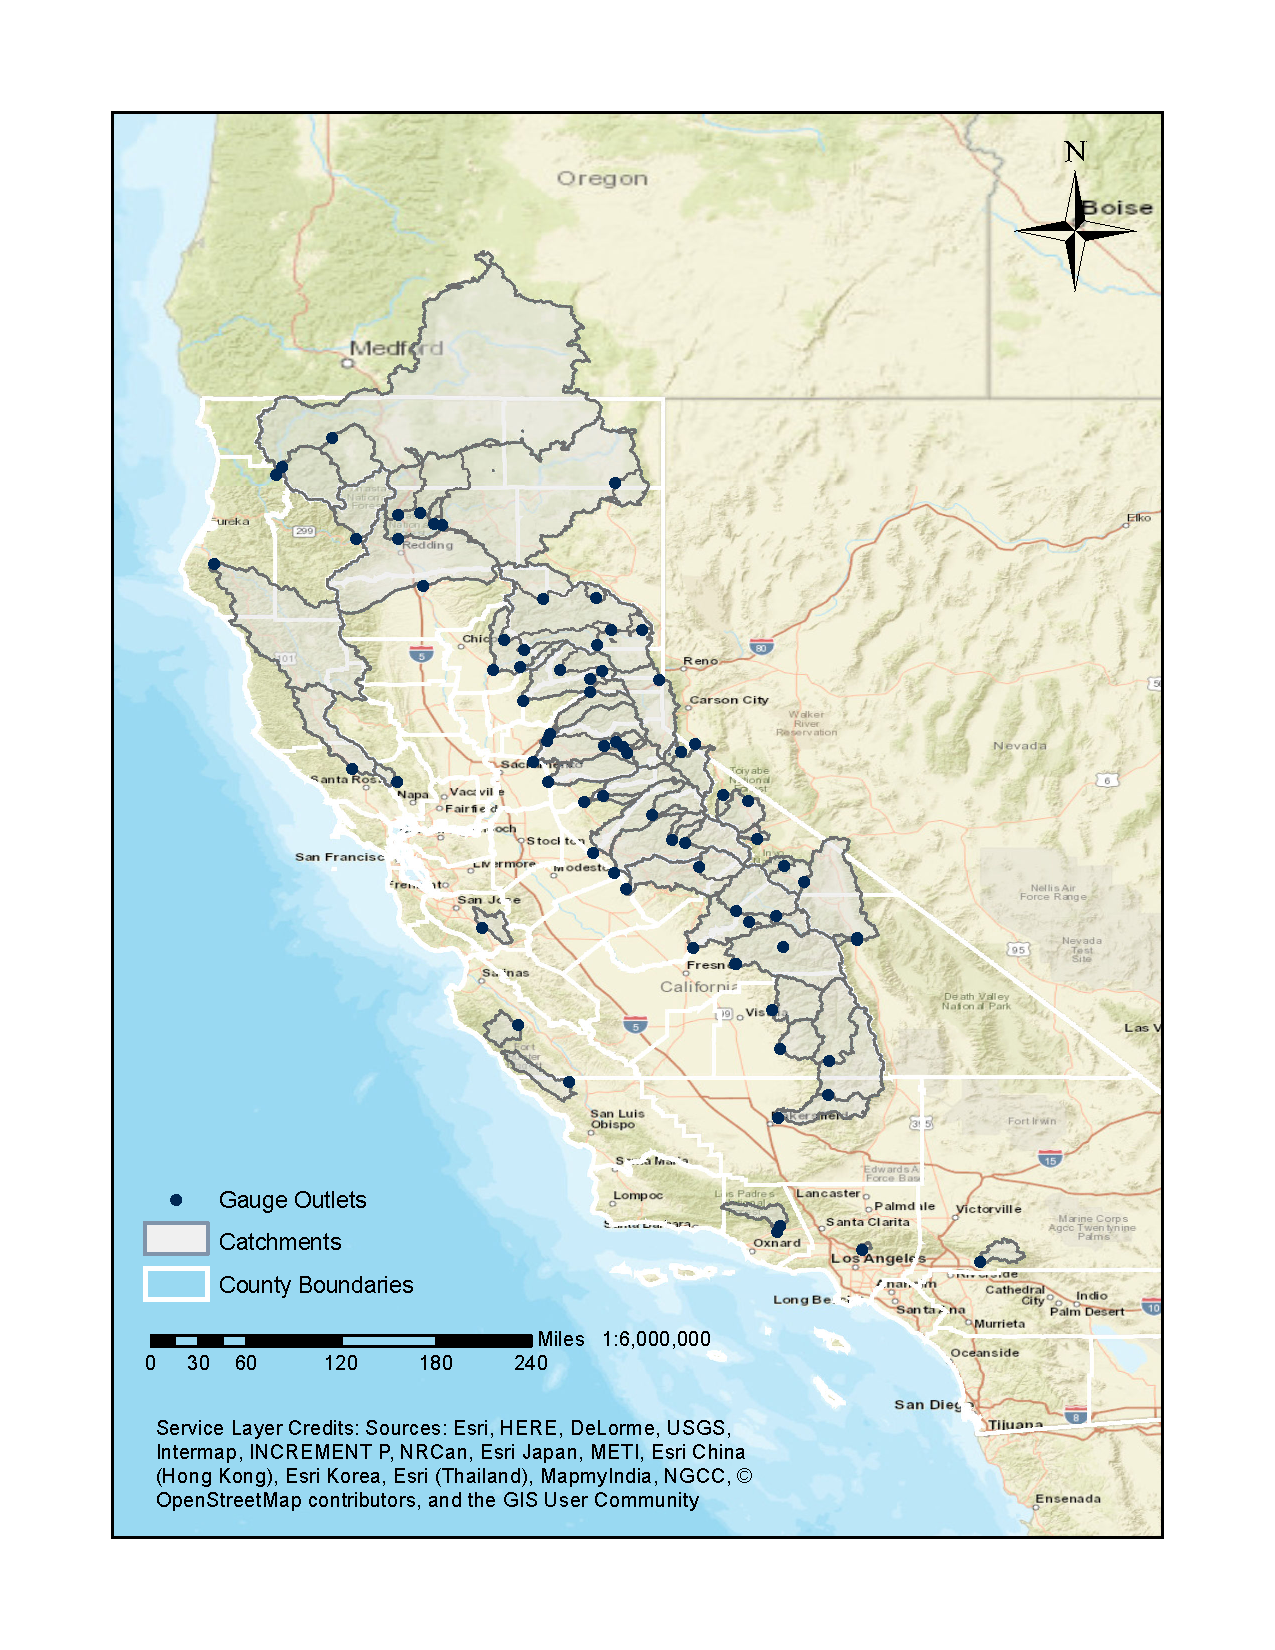
\includegraphics[width=\textwidth,trim={1.5cm 1.5cm 1.5cm 1.5cm},clip=true]{plots/watersheds.pdf}
	\caption{The 67 California basins under study are the CDEC unimpaired flow basins.} 
	\label{fig:map}
\end{figure}

\begin{figure}
	\centering
	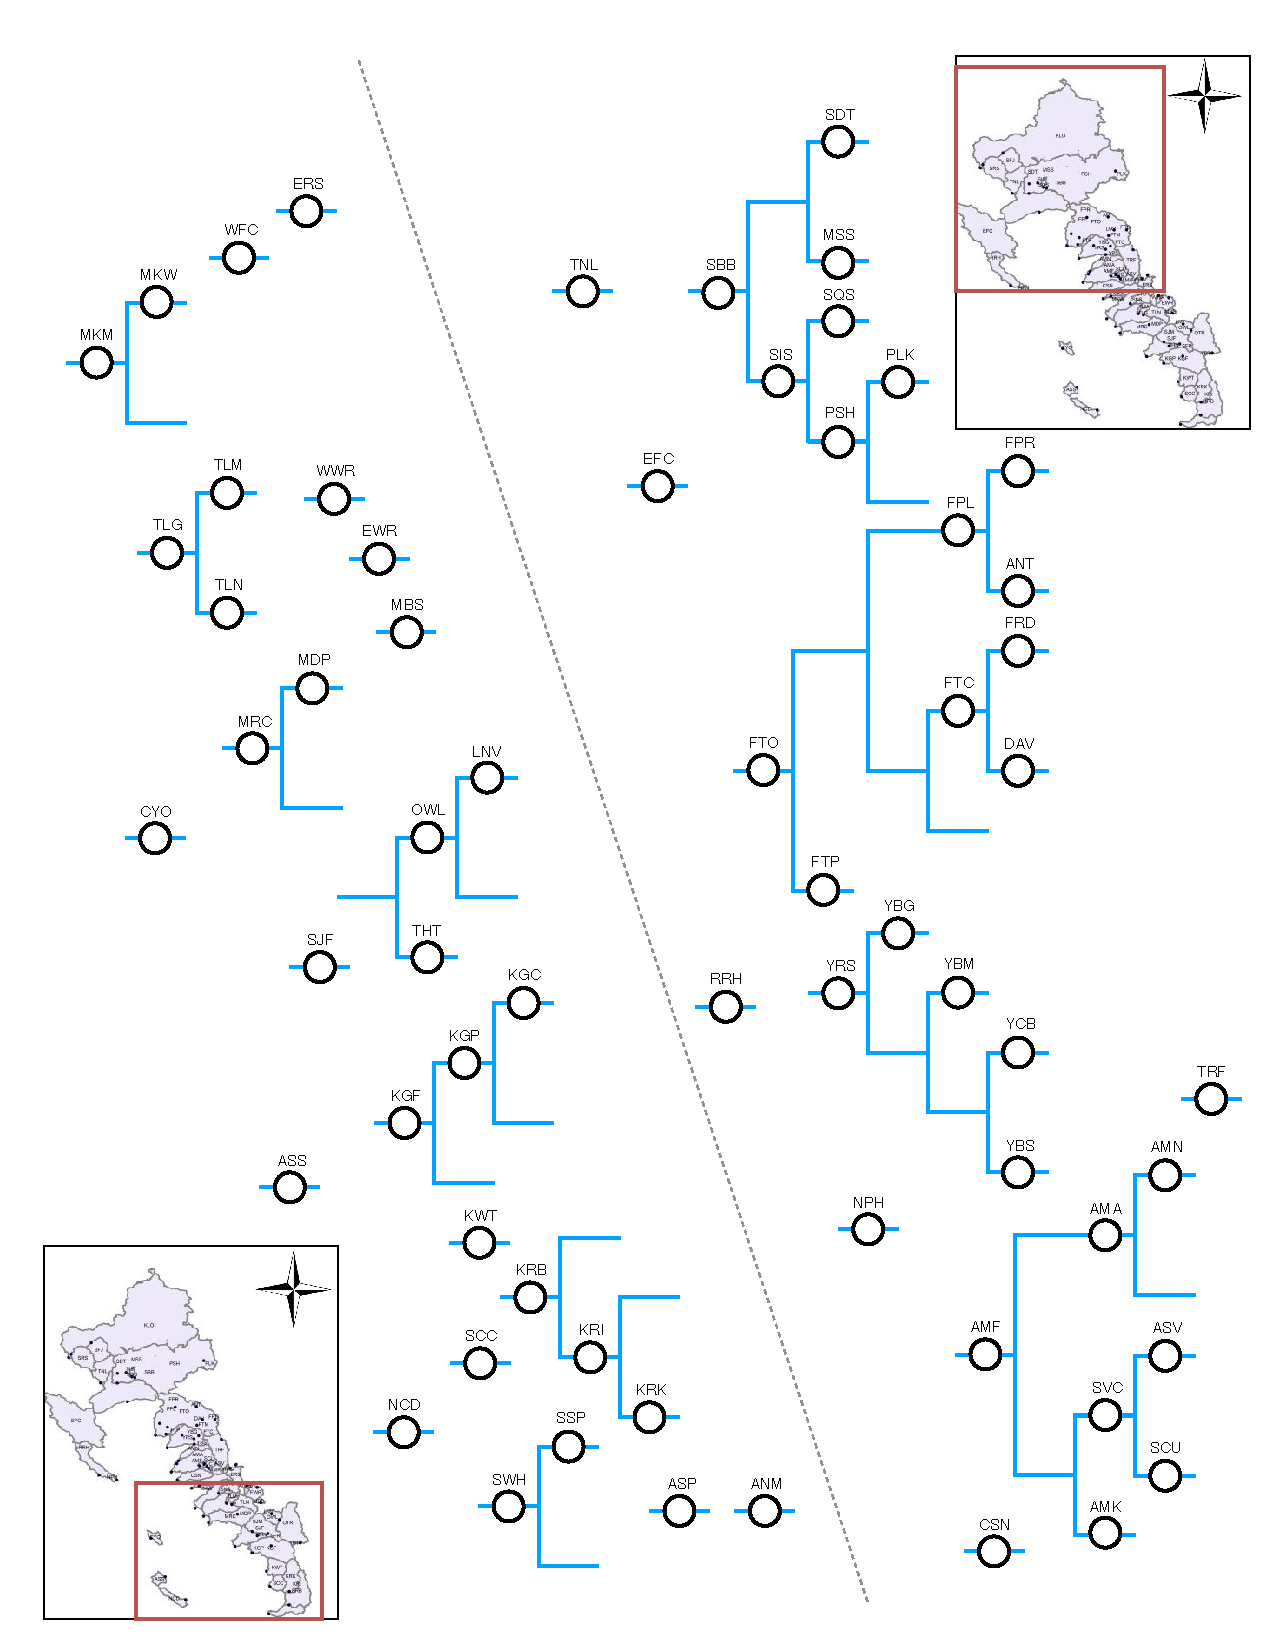
\includegraphics[width=\textwidth,trim={1.5cm 1.5cm 1.5cm 1.5cm},clip=true]{plots/cdecnetwork.pdf}
	\caption{Network schematic.} 
	\label{fig:newtorkmap}
\end{figure}

\begin{figure}
	\centering
	\begin{subfigure}{.5\textwidth}
  		\centering
 		 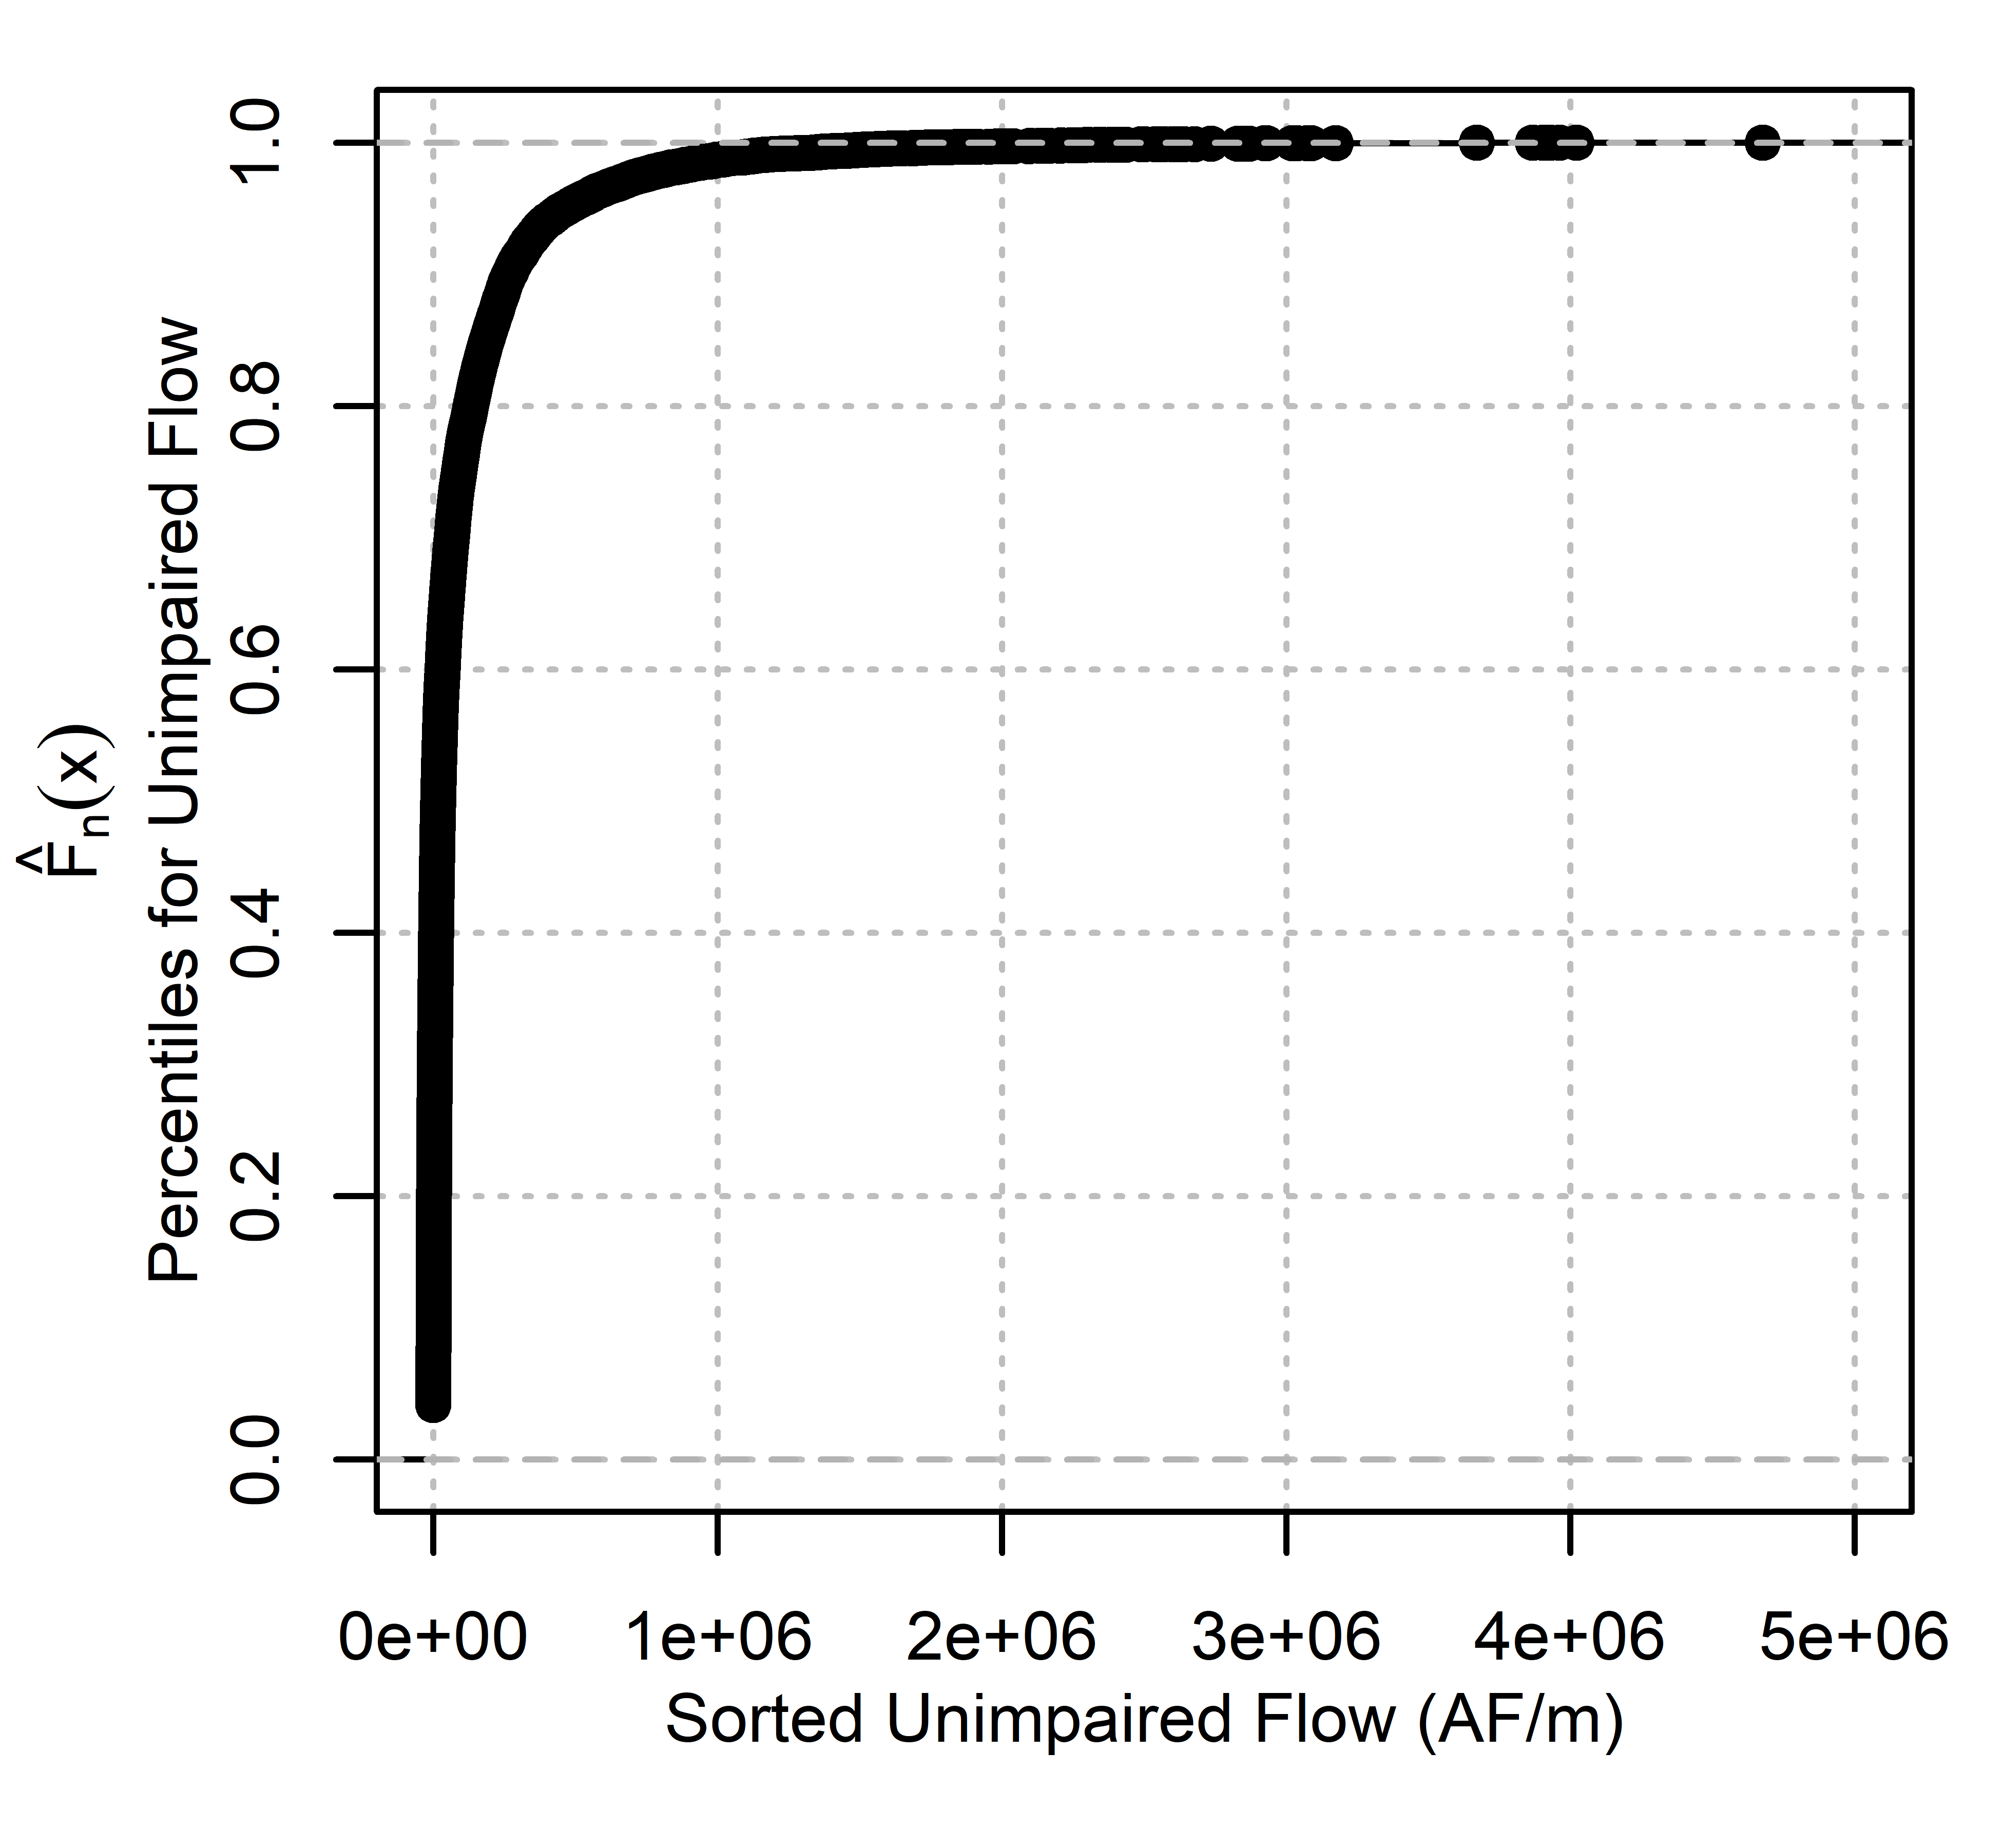
\includegraphics[width=\textwidth, trim={0 0 0 0}, clip=true]{plots/rplot01_flowcdf2.png}
  		\caption{The cumulative distribution function. \newline}
  		\label{fig:flowcdf}
	\end{subfigure}% 
	\begin{subfigure}{.5\textwidth}
  		\centering
  		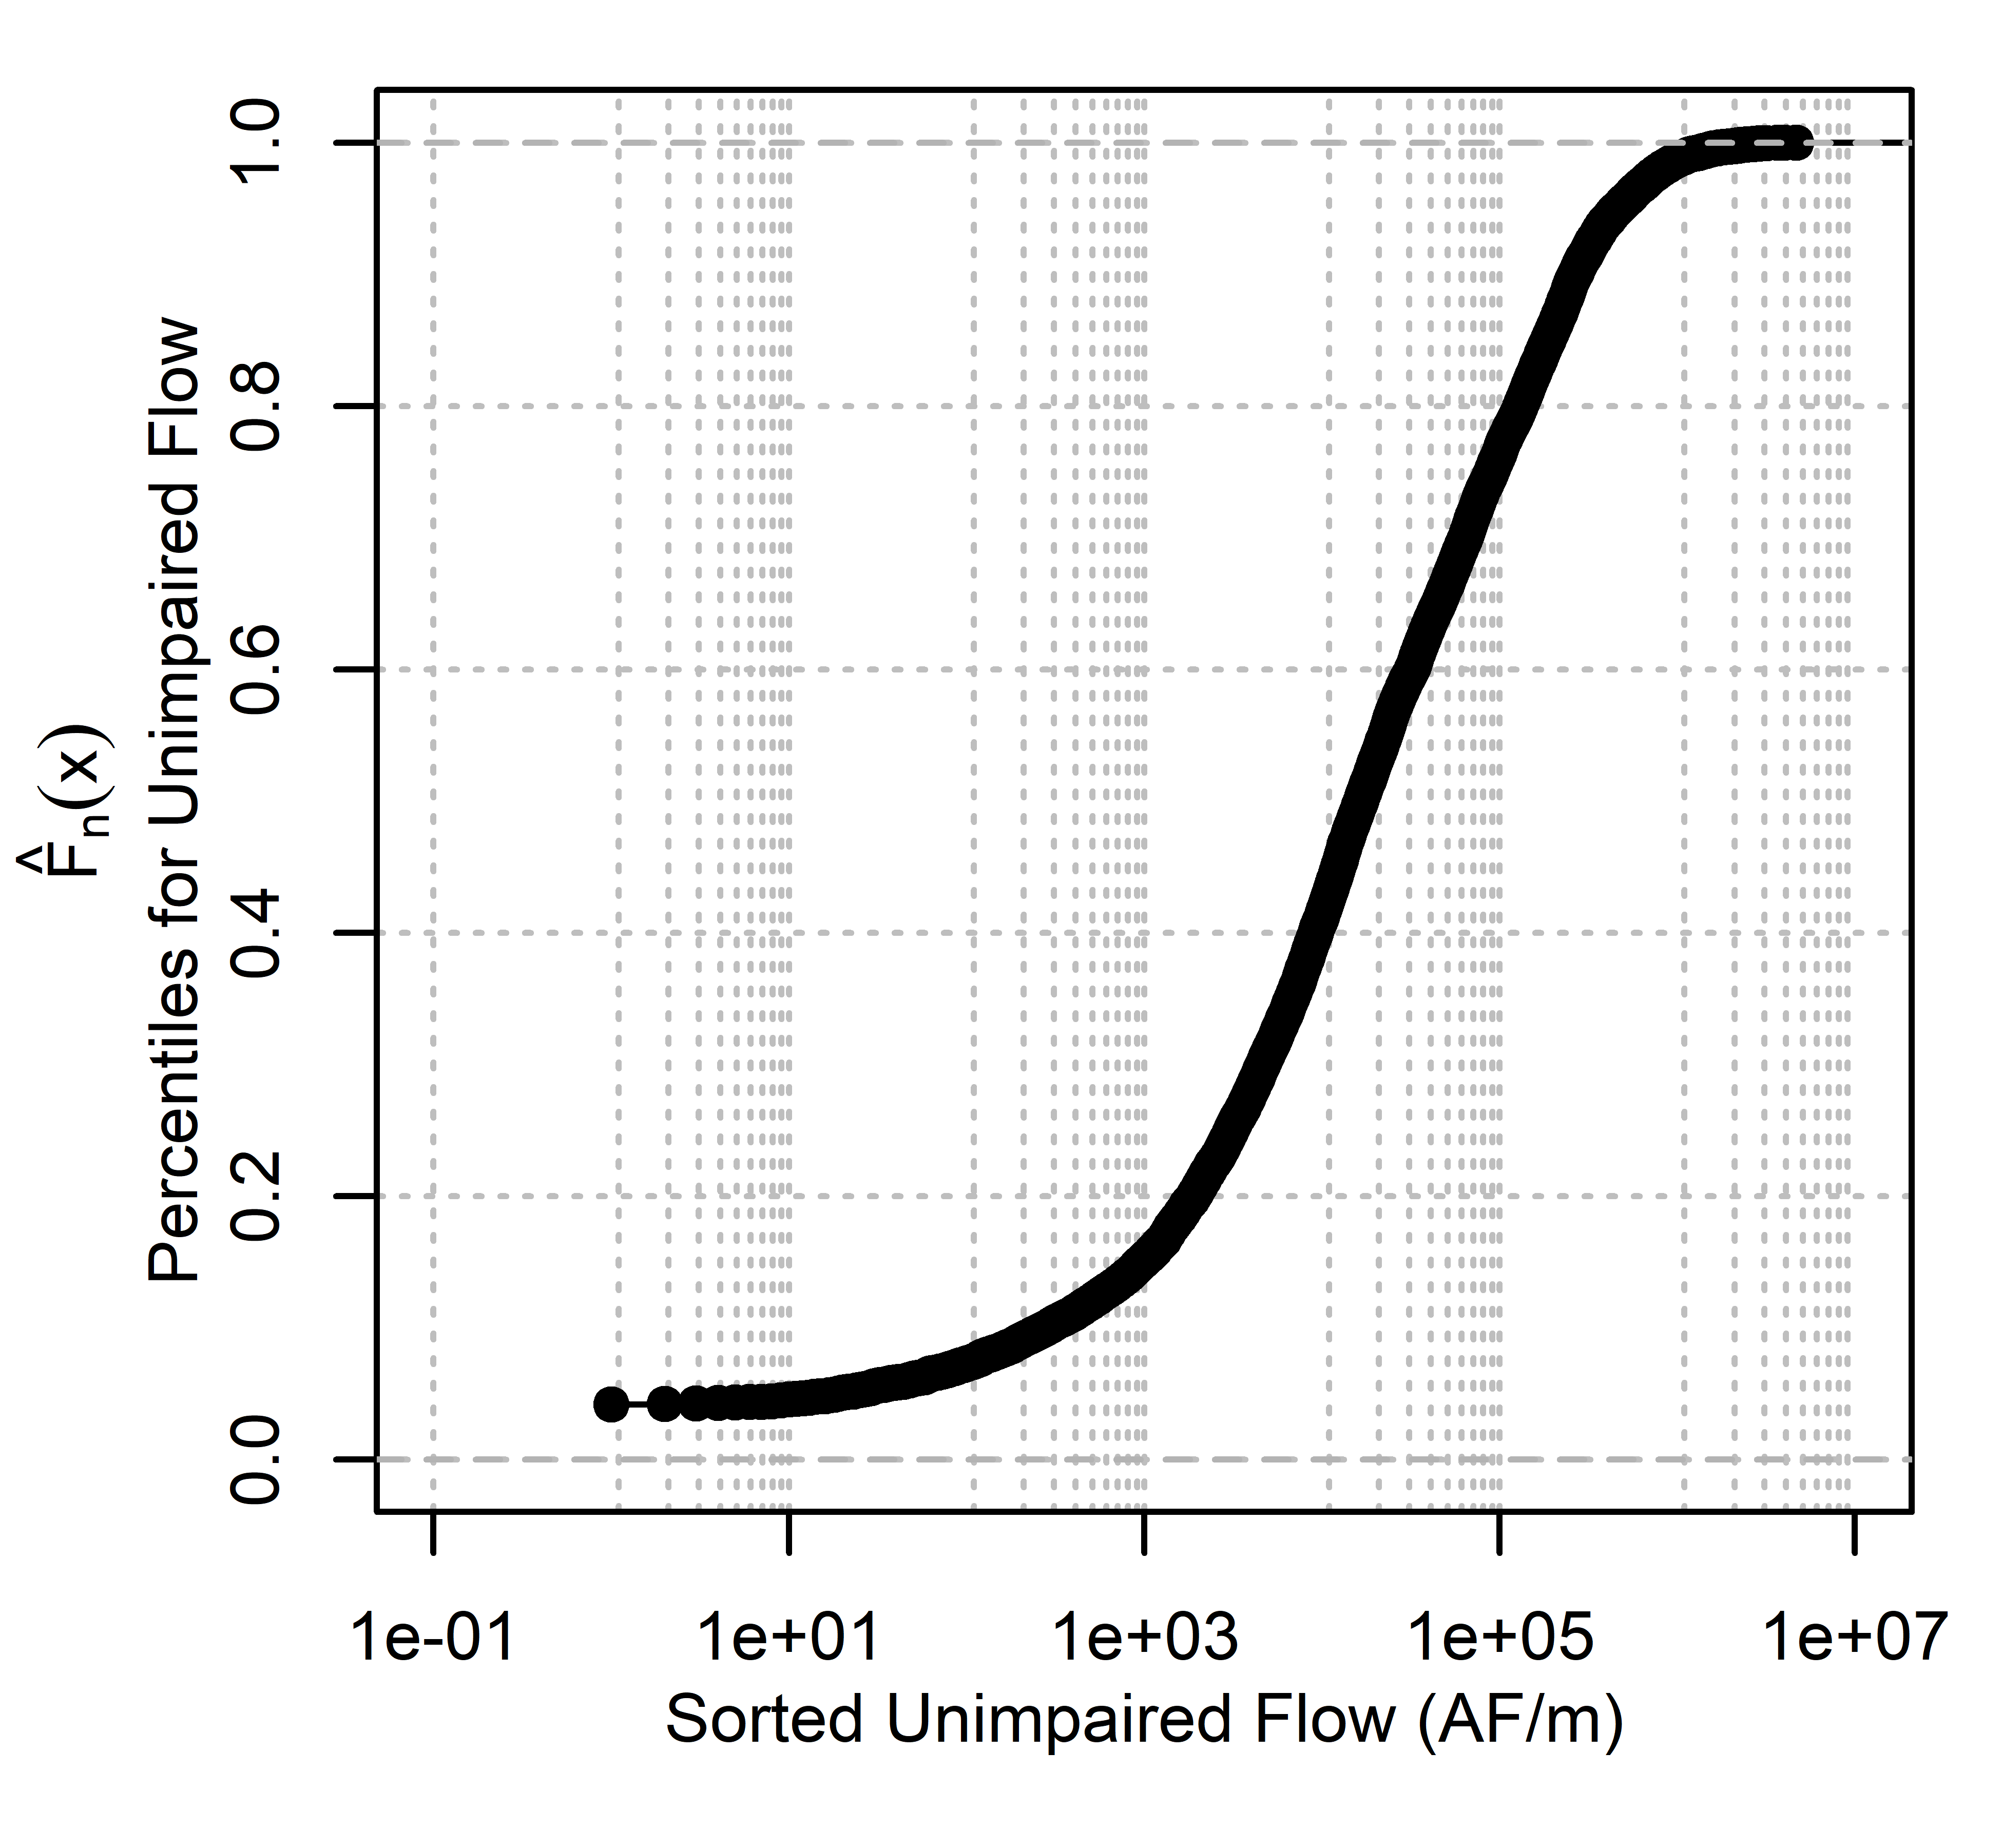
\includegraphics[width=\textwidth, trim={0 0 0 0}, clip=true]{plots/rplot01_flowcdf.png}
  		\caption{The cumulative distribution function in log space.}
  		\label{fig:histkdp}
	\end{subfigure}
	\caption{Distributions of the response variable. Approximately 19,000 unimpaired flows in acre-feet/month.}
	\label{fig:flows}
\end{figure}

% put picture of network here when it's done

%----------------------------------------------------------------------------------------------------------------------------------------------------------------------------------------------------------
\section*{Predictor Variables}
%Precipitation volumes
%Evaporation volumes (Hrachowitz, 2009) → estimates from simple temperature based methods will do (Oudin, 2005) 
%Antecedent wetness (Meyeles, 2003; McDonnell, 2010)
%Precipitation intensity (Blume, 2007; Harchowitz, 2011)
%Stream network connectivity (Jencso, 2009)
%Storm and inter-storm duration (Carillo, 2011)
%Spatial distribution on headwater storage (Spence, 2007) → where water is stored and how accessible the storage is to the outlet
%Drainage density
%Permeability and storage capacity of soil and bedrock
%Height above nearest drainage (Renno, 2008)

Predictor attributes were calculated for each observation point (See Table \ref{table:ufvariables}). A total of 24 predictor variables were selected based on the knowledge of basin characteristics and processes that influence a watershed's response to precipitation: evaporation (temperature); snowfall (cumulative sum of precipitation below 2$^{\circ}$C); storage in soil (with soil and land cover parameters); antecedent conditions (with lagged precipitation and temperature parameters); and groundwater processes (with depth to restricted layer). 

The climate data were derived from the Parameter elevation Regression on Independent Slopes Model (PRISM) dataset, which contains gridded rasters for the continental United States at 4$km$ resolution from 1891 to 2014. The \textbf{temperature} variable and its lagged forms are the basin averaged PRISM \textit{tmean} variable, which in turn was calculated by the mean of the monthly minimum temperatures and the monthly maximum temperatures. The \textbf{precipitation} variable and its lagged forms are the basin averaged PRISM \textit{ppt} variable, which is a measure of total precipitation (rain and snow). 

Low flows in some Sierra Nevada basins exhibit a ``memory'' effect in which they depend on the current and previous year's snowpack \cite{godsey2014effects}. Since we did not want to include 24 lagged precipitation parameters in the model, we developed a snow variable. The \textbf{snow} variable was the cumulative sum of precipitation, starting in October of each water year, for temperatures under 2$^{\circ}$C. 

Basin shape can affect the peak discharge; peak discharge for a circular basin arrives sooner than for an elongated basin of the same area. Because of how the tributary network in a circular basin is organized, the flows in a circular basin enter the main stem at roughly the same time, so more runoff is delivered to the outlet together, sooner. In an elongated basin, because of the mismatch in timing, peak runoff is more attenuated, except for some slow moving streams. The \textbf{shape} parameter, calculated by basin length divided by basin width, and the \textbf{compactness} parameter, calculated by basin area divided by (basin perimeter)$^2$, account for this phenomenon. Although, this phenomenon is more pronounced in runoff on a smaller time step, we included these parameters in the final model to see their importance. 

Basin hypsometric information was derived from the Shuttle Radar Topography Mission (SRTM) 90$m$ model, which is a gridded raster of static elevation at a 3$arc-second$ resolution. The vertical error of the model is reported to be less than 16$m$. The \textbf{mean basin elevation} and \textbf{basin relief ratio} parameters \cite{pike1971elevation} were calculated from this dataset. Basin relief ratio is calculated by the difference in maximum and minimum elevations divided by basin length. 

Soil properties were derived from the POLARIS dataset, a Soil Survey Geographic Database (SSURGO) processed dataset at a 3$arc-second$ resolution. Percent \textbf{clay}, \textbf{silt}, and \textbf{sand}, \textbf{saturated hydraulic conductivity}, \textbf{lambda} and \textbf{n} pore size, \textbf{available water content}, and \textbf{depth to restricted layer} information was averaged for each basin. 

% I deleted this from the model
% The land cover property was derived from the California Vegetation (CALVEG) dataset, which includes the following land cover types: urban (URB), barren (BAR), shrub (SHB), conifers (CON), hardwoods (HDW), water (WAT), mix (MIX) and agriculture (AGR). The \textbf{percent vegetated} parameter, is the percent of land in a basin that is not covered by URB, BAR, and WAT. The \textbf{dominant basin geology} parameter taken from the Natural Resources Conservation Service (NRCS) dataset \textit{rocktype2} variable. Here, the percent of basin area in each rock type category was calculated and the dominant class is preserved. \\

\begingroup
	\renewcommand{\arraystretch}{1.2} 
	\linespread{1.0}
	\footnotesize 
	\centering
	\captionof{table}{Summary of the variables used in the implementation of the model.} 
	\begin{longtable}[h]{p{2cm}p{2.55cm}p{8.04cm}p{2.24cm}}
%\begin{table*}[h]\renewcommand{\arraystretch}{1.2} 
%	\linespread{1.0}
%	\footnotesize
%	\centering
%	\caption{Summary of the variables used in the implementation of the model.}
%	\begin{tabular}{p{2cm}p{2.55cm}p{8.04cm}p{2.24cm}} % must add to 16.5
	Type & Variable & Description & Source \\
	\hline
	\endhead
	Response & Unimpaired Flow & monthly estimated unimpaired flows, in $AF$ & CDEC \cite{beaudette2016package} \\
	\hline
	% Time & Month & categorical: Jan, Feb, ..., Dec & - \\
	Time & Ordinal Month & numerical distance till October & \\
	% & Season & categorical: Fall, Winter, Spring, Summer & \\
	& Water Year & numeric year starting from the October of previous Gregorian year & \\
	\hline
	Climate & Temperature, Lag 1, 2 and 3 Months & temperature and lagged monthly temperature, in $^{\circ}$C & PRISM  \cite{prism} \\
	& Precipitation, Lag 1, 2 and 3 Months & precipitation and lagged monthly precipitation, in $mm$ &  \\  
	& Snow & cumulative precipitation of the same water year for temperatures bellow 2 $^{\circ}$C, in $mm$& \\
	\hline
	Hypsometric & Relief Ratio & (max(elev) - min(elev))/ basin length in, $m/m$ & SRTM90 \cite{jarvis2008hole}\\
	& Mean Elevation & mean basin elevation, in $m$ & \\
	\hline
	Basin Boundaries & Area & basin drainage area, in $m^2$ & NHD2PLUS \cite{mckay2012nhdplus}\\
	& Shape & basin length/basin width, in $m/m$ &  \\
	 & Compactness & basin area/(basin perimeter)$^2$, in $m^2/m^2$ &  \\
	\hline
	Soil & \% Clay & percent clay in surface layer, in $\%$ & POLARIS \cite{chaney2016polaris} \\
	 & \% Silt & percent silt in surface layer, in $\%$ &  \\
	 & \% Sand & percent sand in surface layer, in $\%$ &  \\
	 & Sat. Hydraulic Conductivity & hydrologic conductivity of surface layer, in $cm$/$hr$ &  \\
	 & Lambda & pore size distribution index (brooks-corey) & \\
	 & N & measure of the pore size distribution (van genuchten) & \\
	 & Available water content & available water content, in $m^3/m^3$ & \\ 
	\hline
	Land Cover & Vegetated & Percent of area in the basin vegetated in $\%$ & CALVEG \cite{calveg2004vegetation} \\
	\hline
	%Ground Water & Dominant Geology & dominant rock type in basin, categorical & NRCS \cite{nrcs2006land} \\
	Ground Water & Depth to Restricted Layer & depth to aquitard, in $cm$ & POLARIS \cite{chaney2016polaris}\\
%	\hline 
%	\end{tabular}
%	\label{table:ufvariables}
%\end{table*}
	\hline
	\end{longtable}
	\label{table:ufvariables}
\endgroup

%----------------------------------------------------------------------------------------------------------------------------------------------------------------------------------------------------------
\section*{Other Descriptive Variables}
Some variables are included in the dataset, but not in the modeling; these variables define the location of the guages, and consist of the following: Longitude and Latitude (definite location), Hierarchy or the number of guages that exist above (relative location in the network), river basin, county, and guage operator. These variables are only used for plotting purposes (See Figure \ref{fig:monthlyboxplot}, \ref{fig:flowvslat}, and \ref{fig:flowvsppt}). 

\begin{figure}
	\centering
	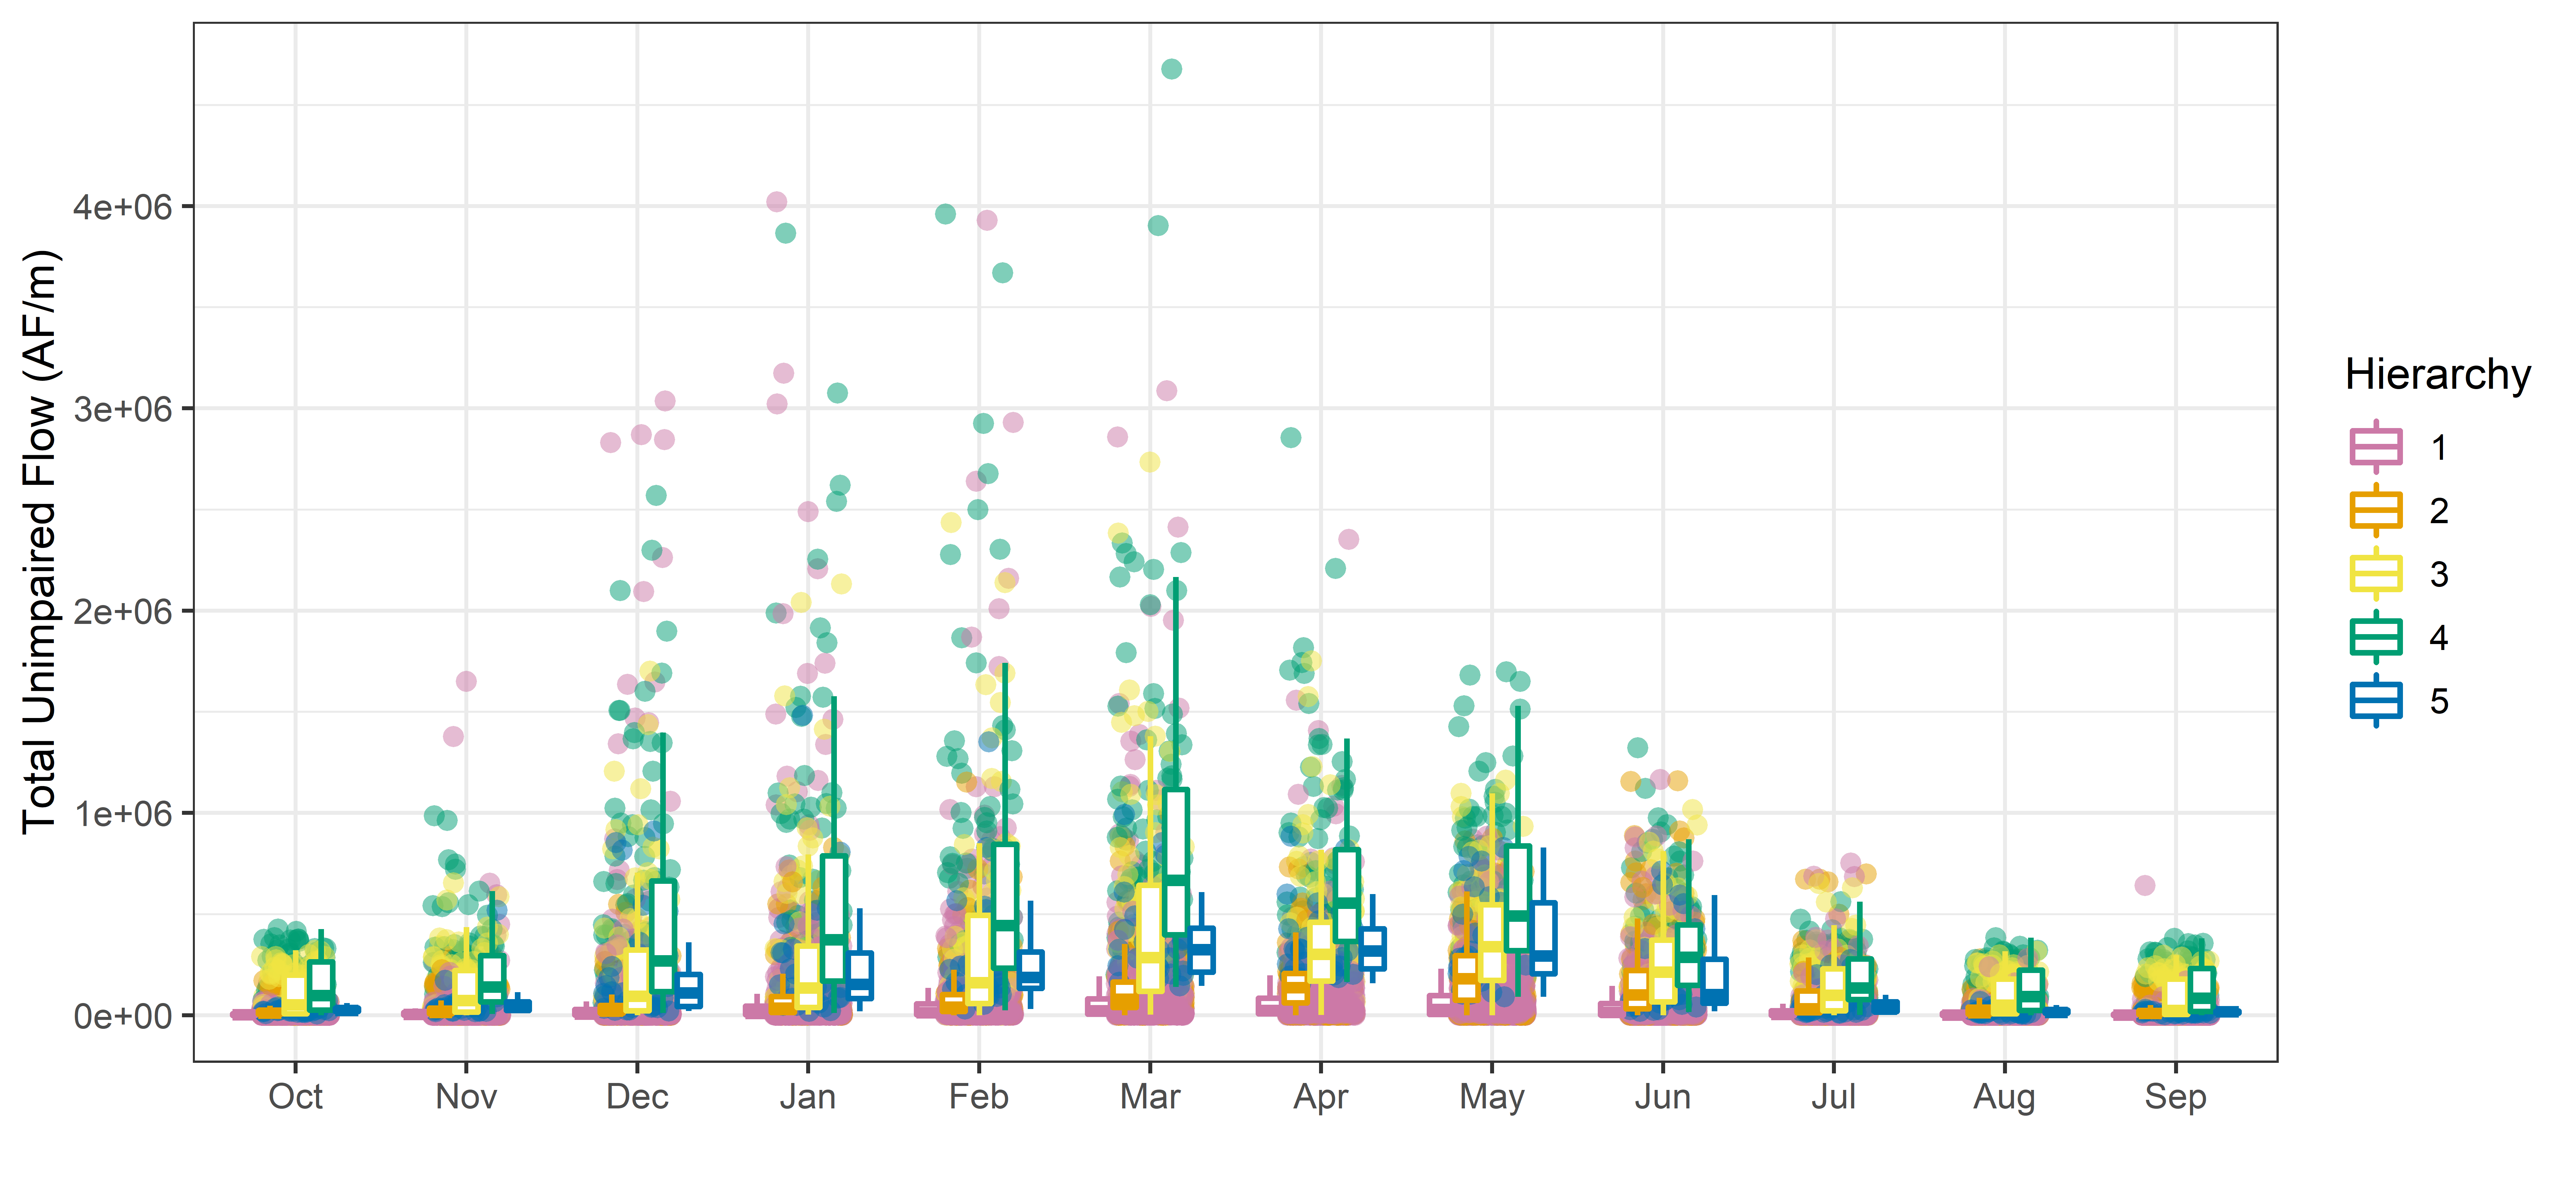
\includegraphics[width=\textwidth, trim={0 0 0 0}, clip=true]{plots/rplot04_boxplot.png}
	\caption{The cyclical behavoir of total monthly unimpaired flows. The flows start to rise in October, the start of the ``water year". The boxplots also show that given a higher hierarchy (i.e., being lower in the network of guages) the monthly distribution of flows becomes larger. The only expection to this is basin hierarchy number 5, and that is due to the fact that this data set only had one basin in that hierarchy. Had there been more basins, its distribution would be wider showing that the lower you are in the network, the higher the flows and the bigger the distribution of flows.} 
	\label{fig:monthlyboxplot}
\end{figure}

\begin{figure}
	\centering
	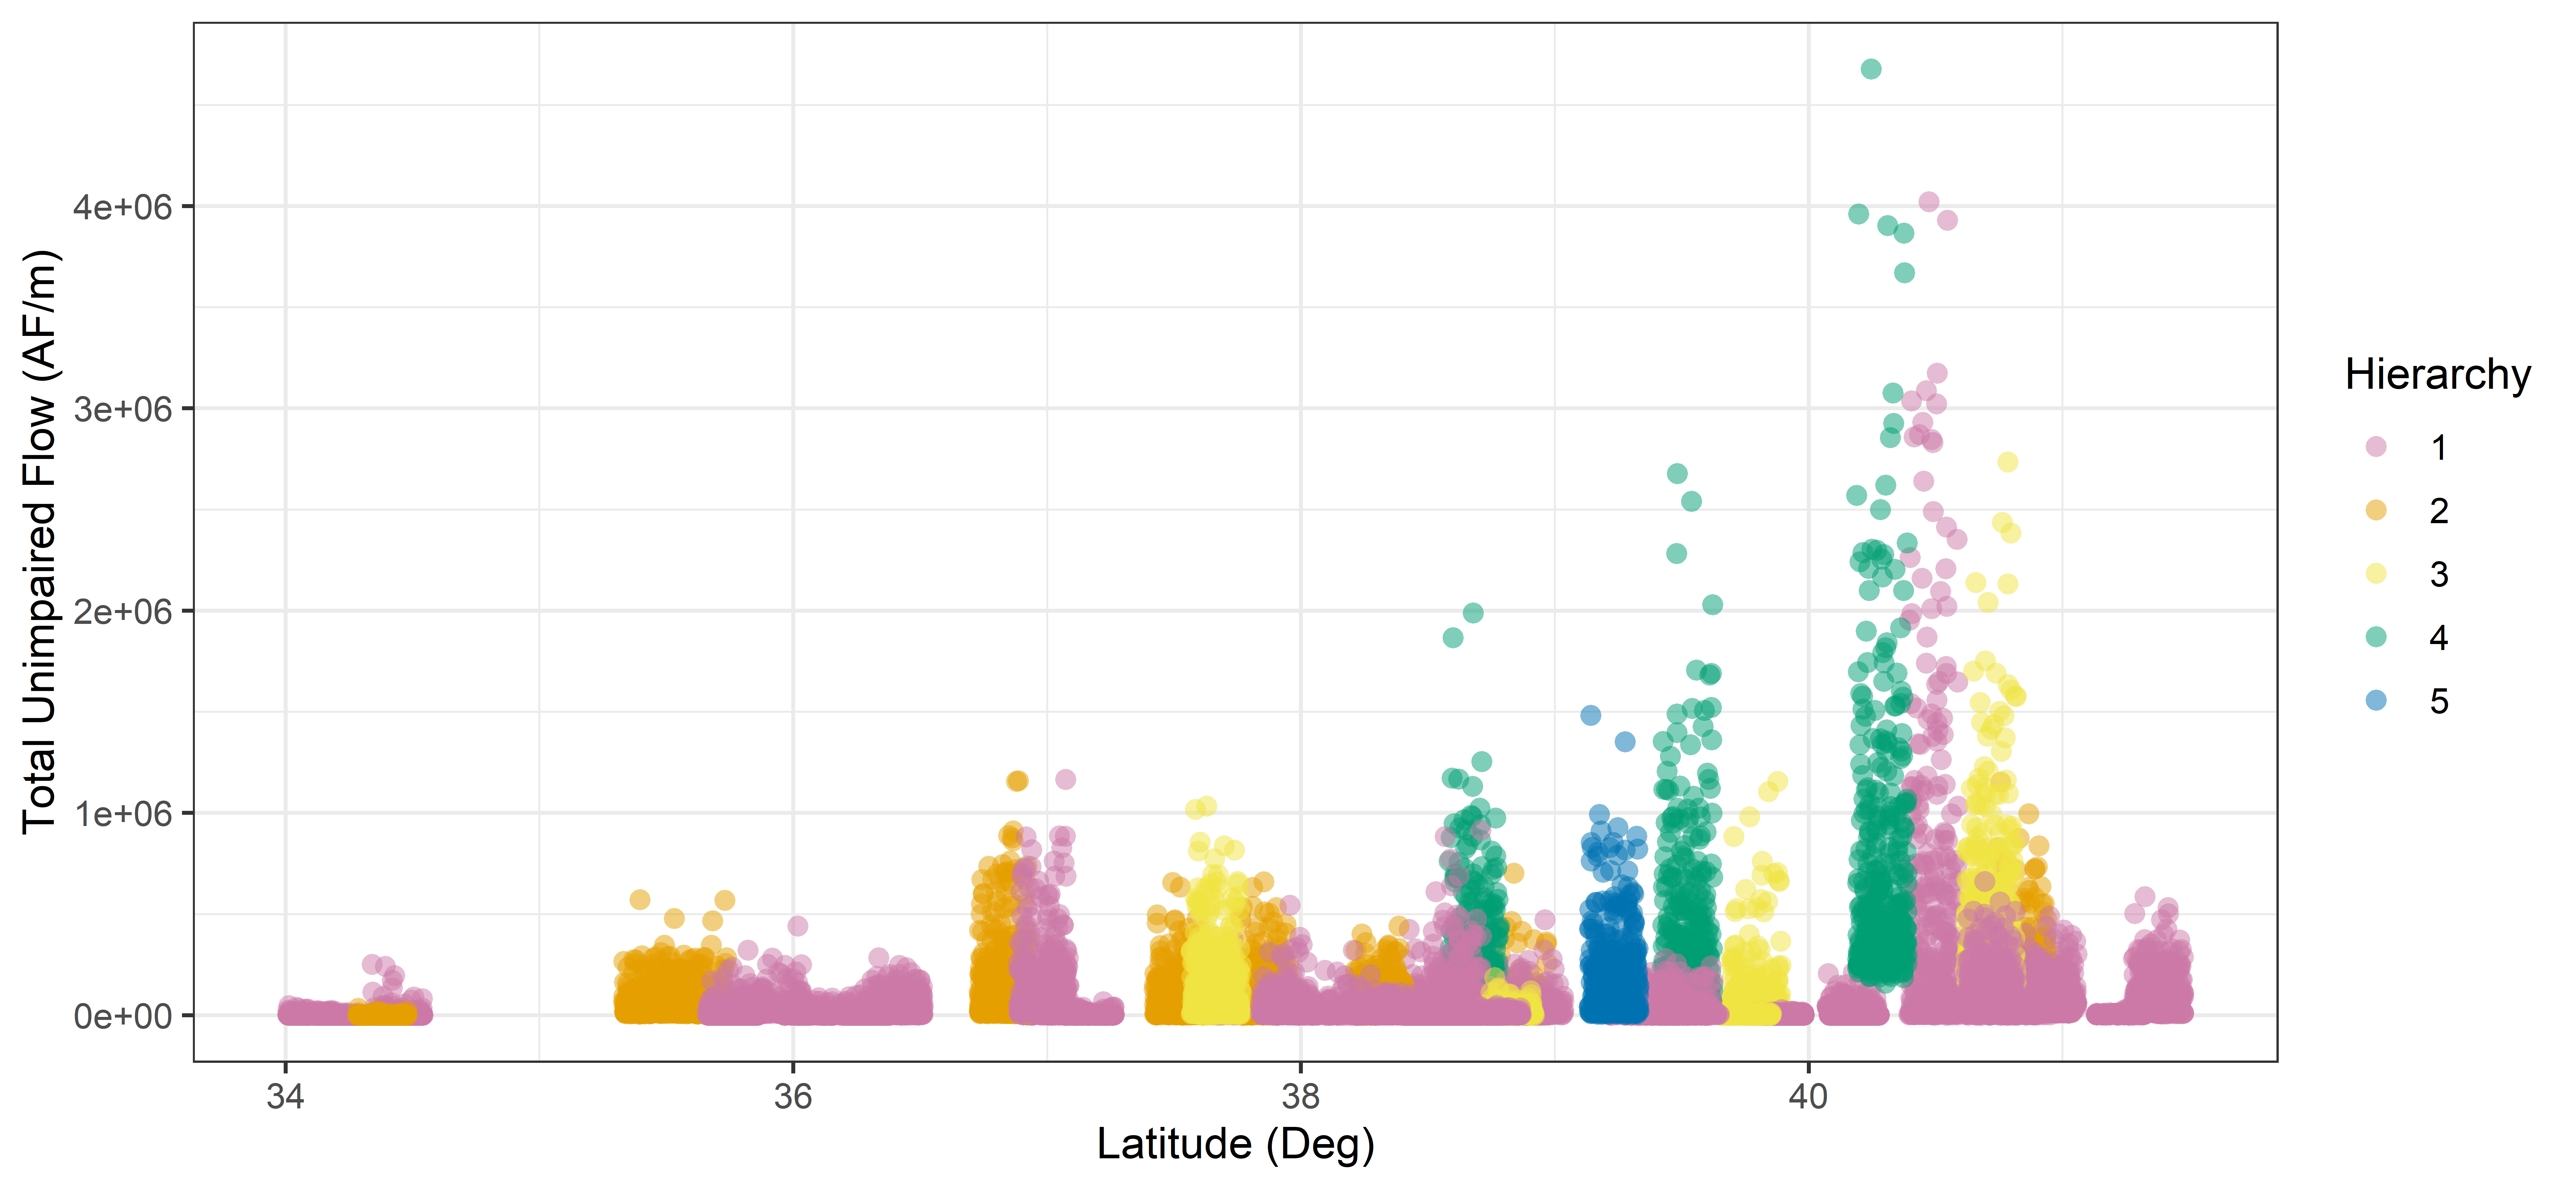
\includegraphics[width=\textwidth, trim={0 0 0 0}, clip=true]{plots/rplot05_flowvslat.png}
	\caption{Total monthly unimpaired flow vs. latitude. Total monthly unimpaierd flow increases at higher latitudes in California. Note that each of the basins were at a unique latitude, for illustration purposes the latitude variable was jittered.} 
	\label{fig:flowvslat}
\end{figure}

\begin{figure}
	\centering
	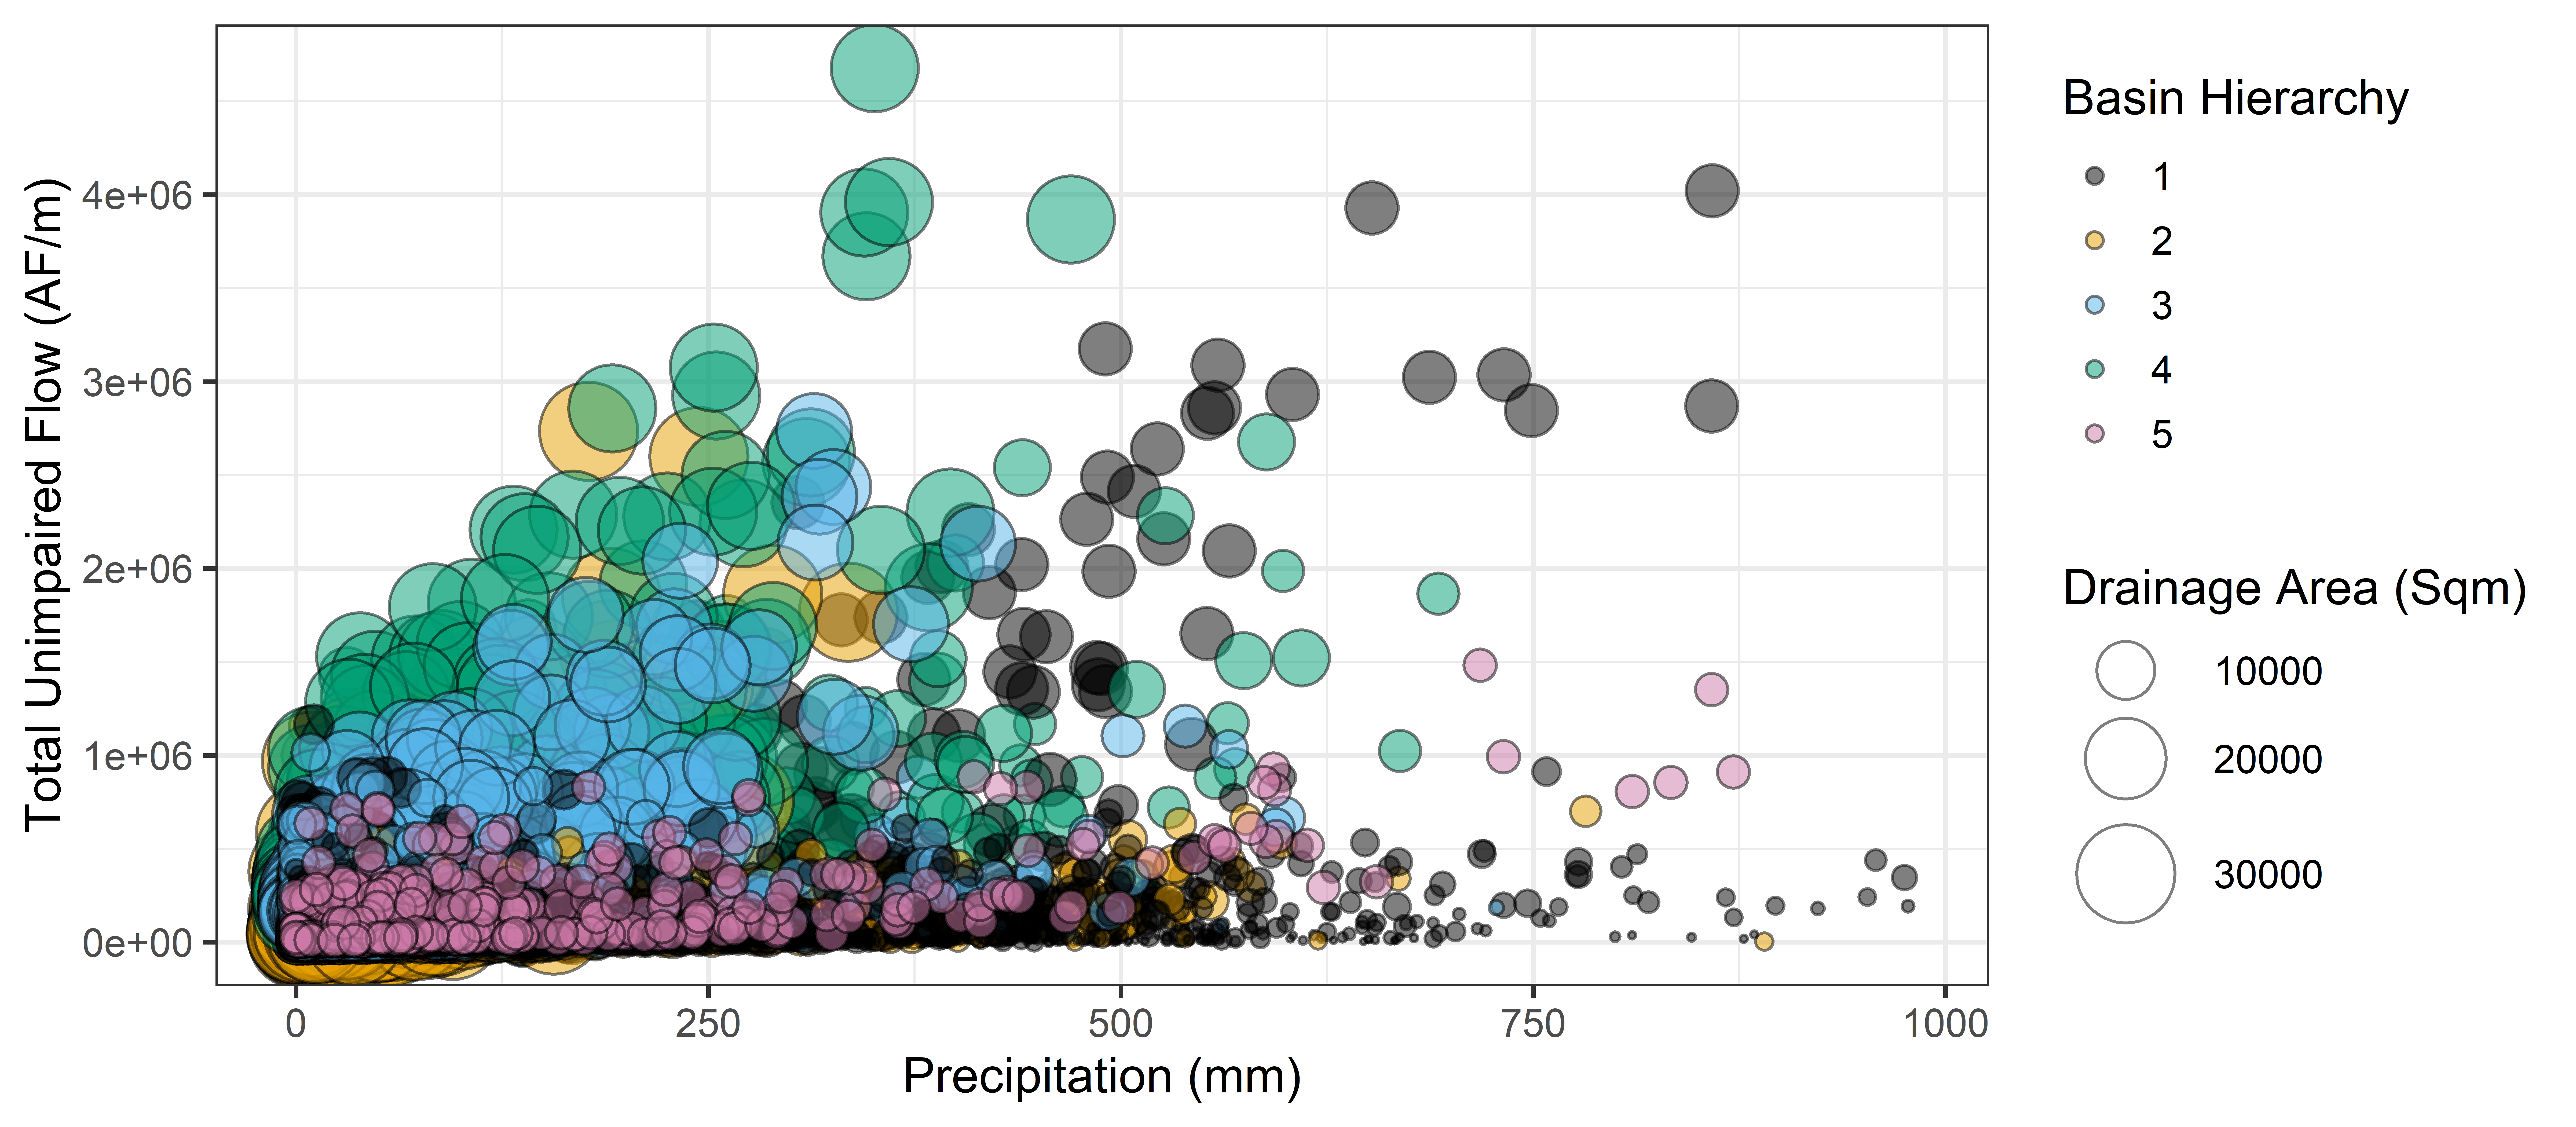
\includegraphics[width=\textwidth, trim={0 0 0 0}, clip=true]{plots/rplot05_pptvsflow.png}
	\caption{Ttoal monthly unimpaired flow vs. precipitation. The total monthly unimpaired flow increases with increasing precipitation. This is also drainage area dependent, as the smaller drainage areas that happen to have high amounts of precipitation still produce low flows. Basin hierarchies also show that the larger basins are lower in the network. The only exepction being hierarchy number 5, and that is due to the fact that this data set only had one basin in that hierarchy.} 
	\label{fig:flowvsppt}
\end{figure}

%----------------------------------------------------------------------------------------------------------------------------------------------------------------------------------------------------------
\section*{Correlations}
A simple examination of the partial correlations of predictor variables with flow shows that most of the information content lies within drainage area, precipitation, and some measures of infiltration (i.e., lambda pore size, n pore size, and saturated hydraulic conductivity). The correlated variables were not removed from the model (See Figure\ref{fig:correlogram}). For a more complete correlation plot see Figure \ref{fig:corrplot}. 

\begin{figure}
	\centering
	\begin{subfigure}{.5\textwidth}
  		\centering
 		 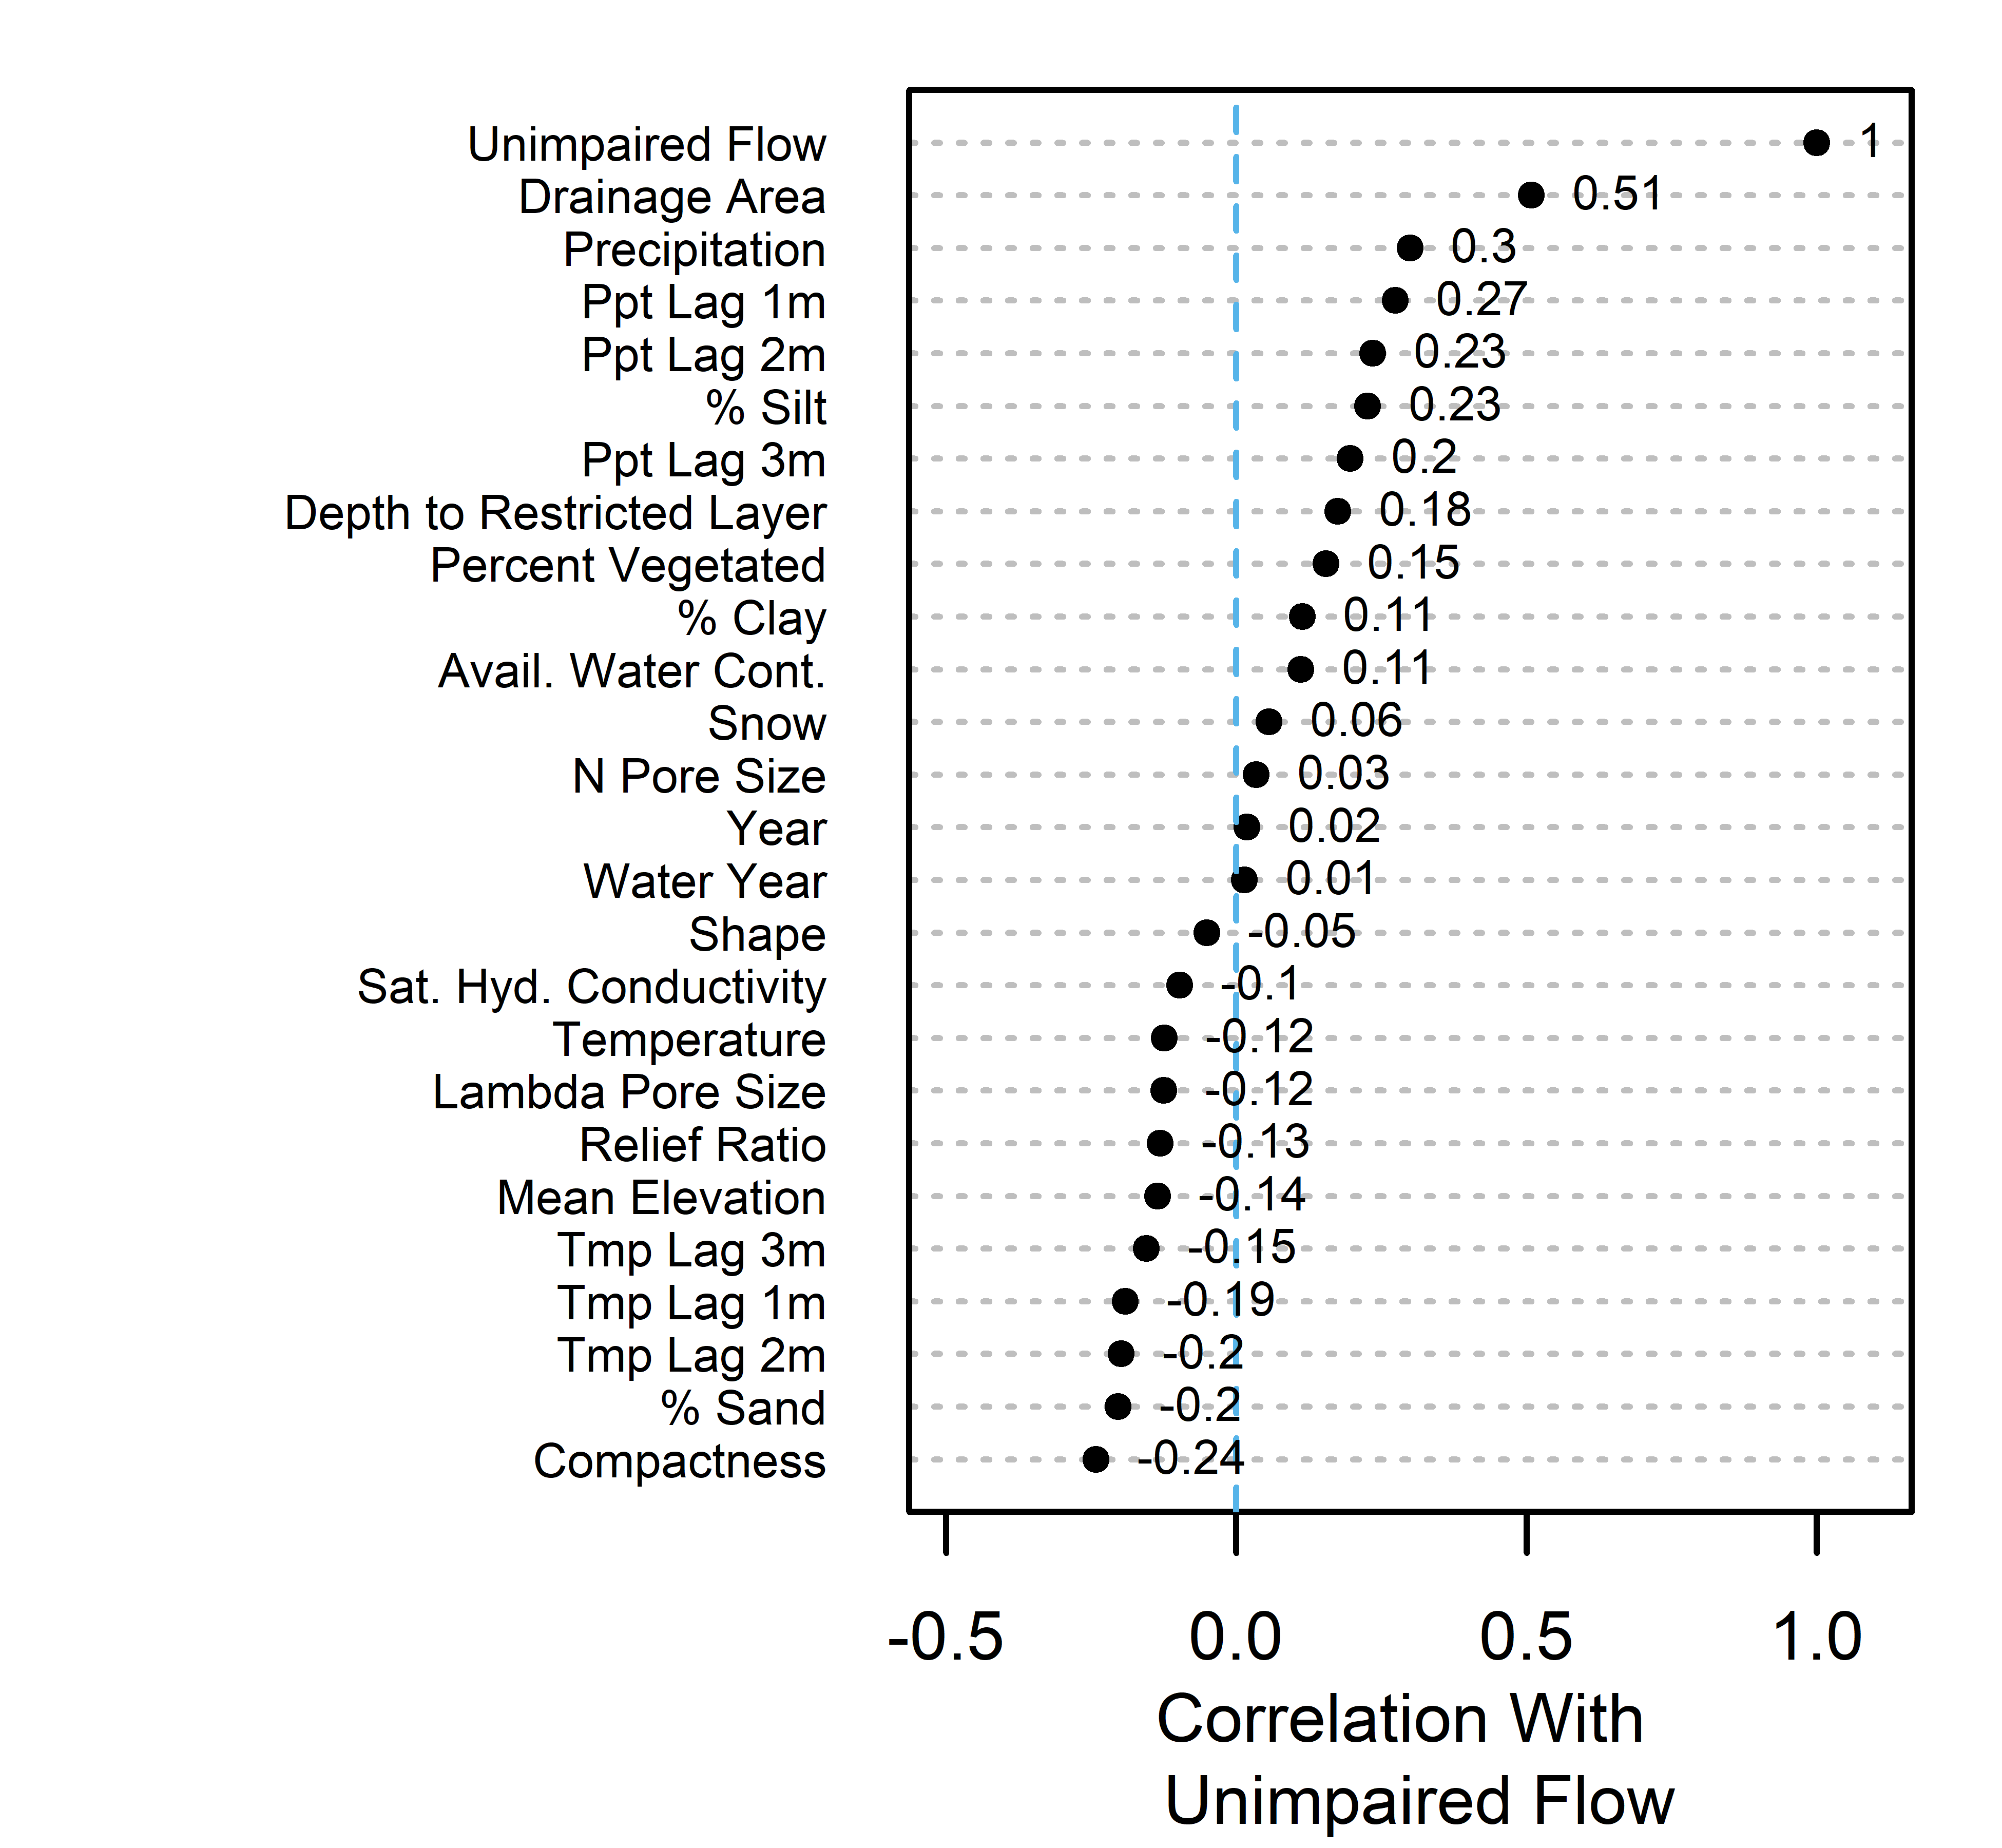
\includegraphics[width=\textwidth, trim={0 0 0 0}, clip=true]{plots/rplot08_corrwithflow.png}
  		\caption{Pearson's Correlation}
  		\label{fig:sub1}
	\end{subfigure}% 
	\begin{subfigure}{.5\textwidth}
  		\centering
  		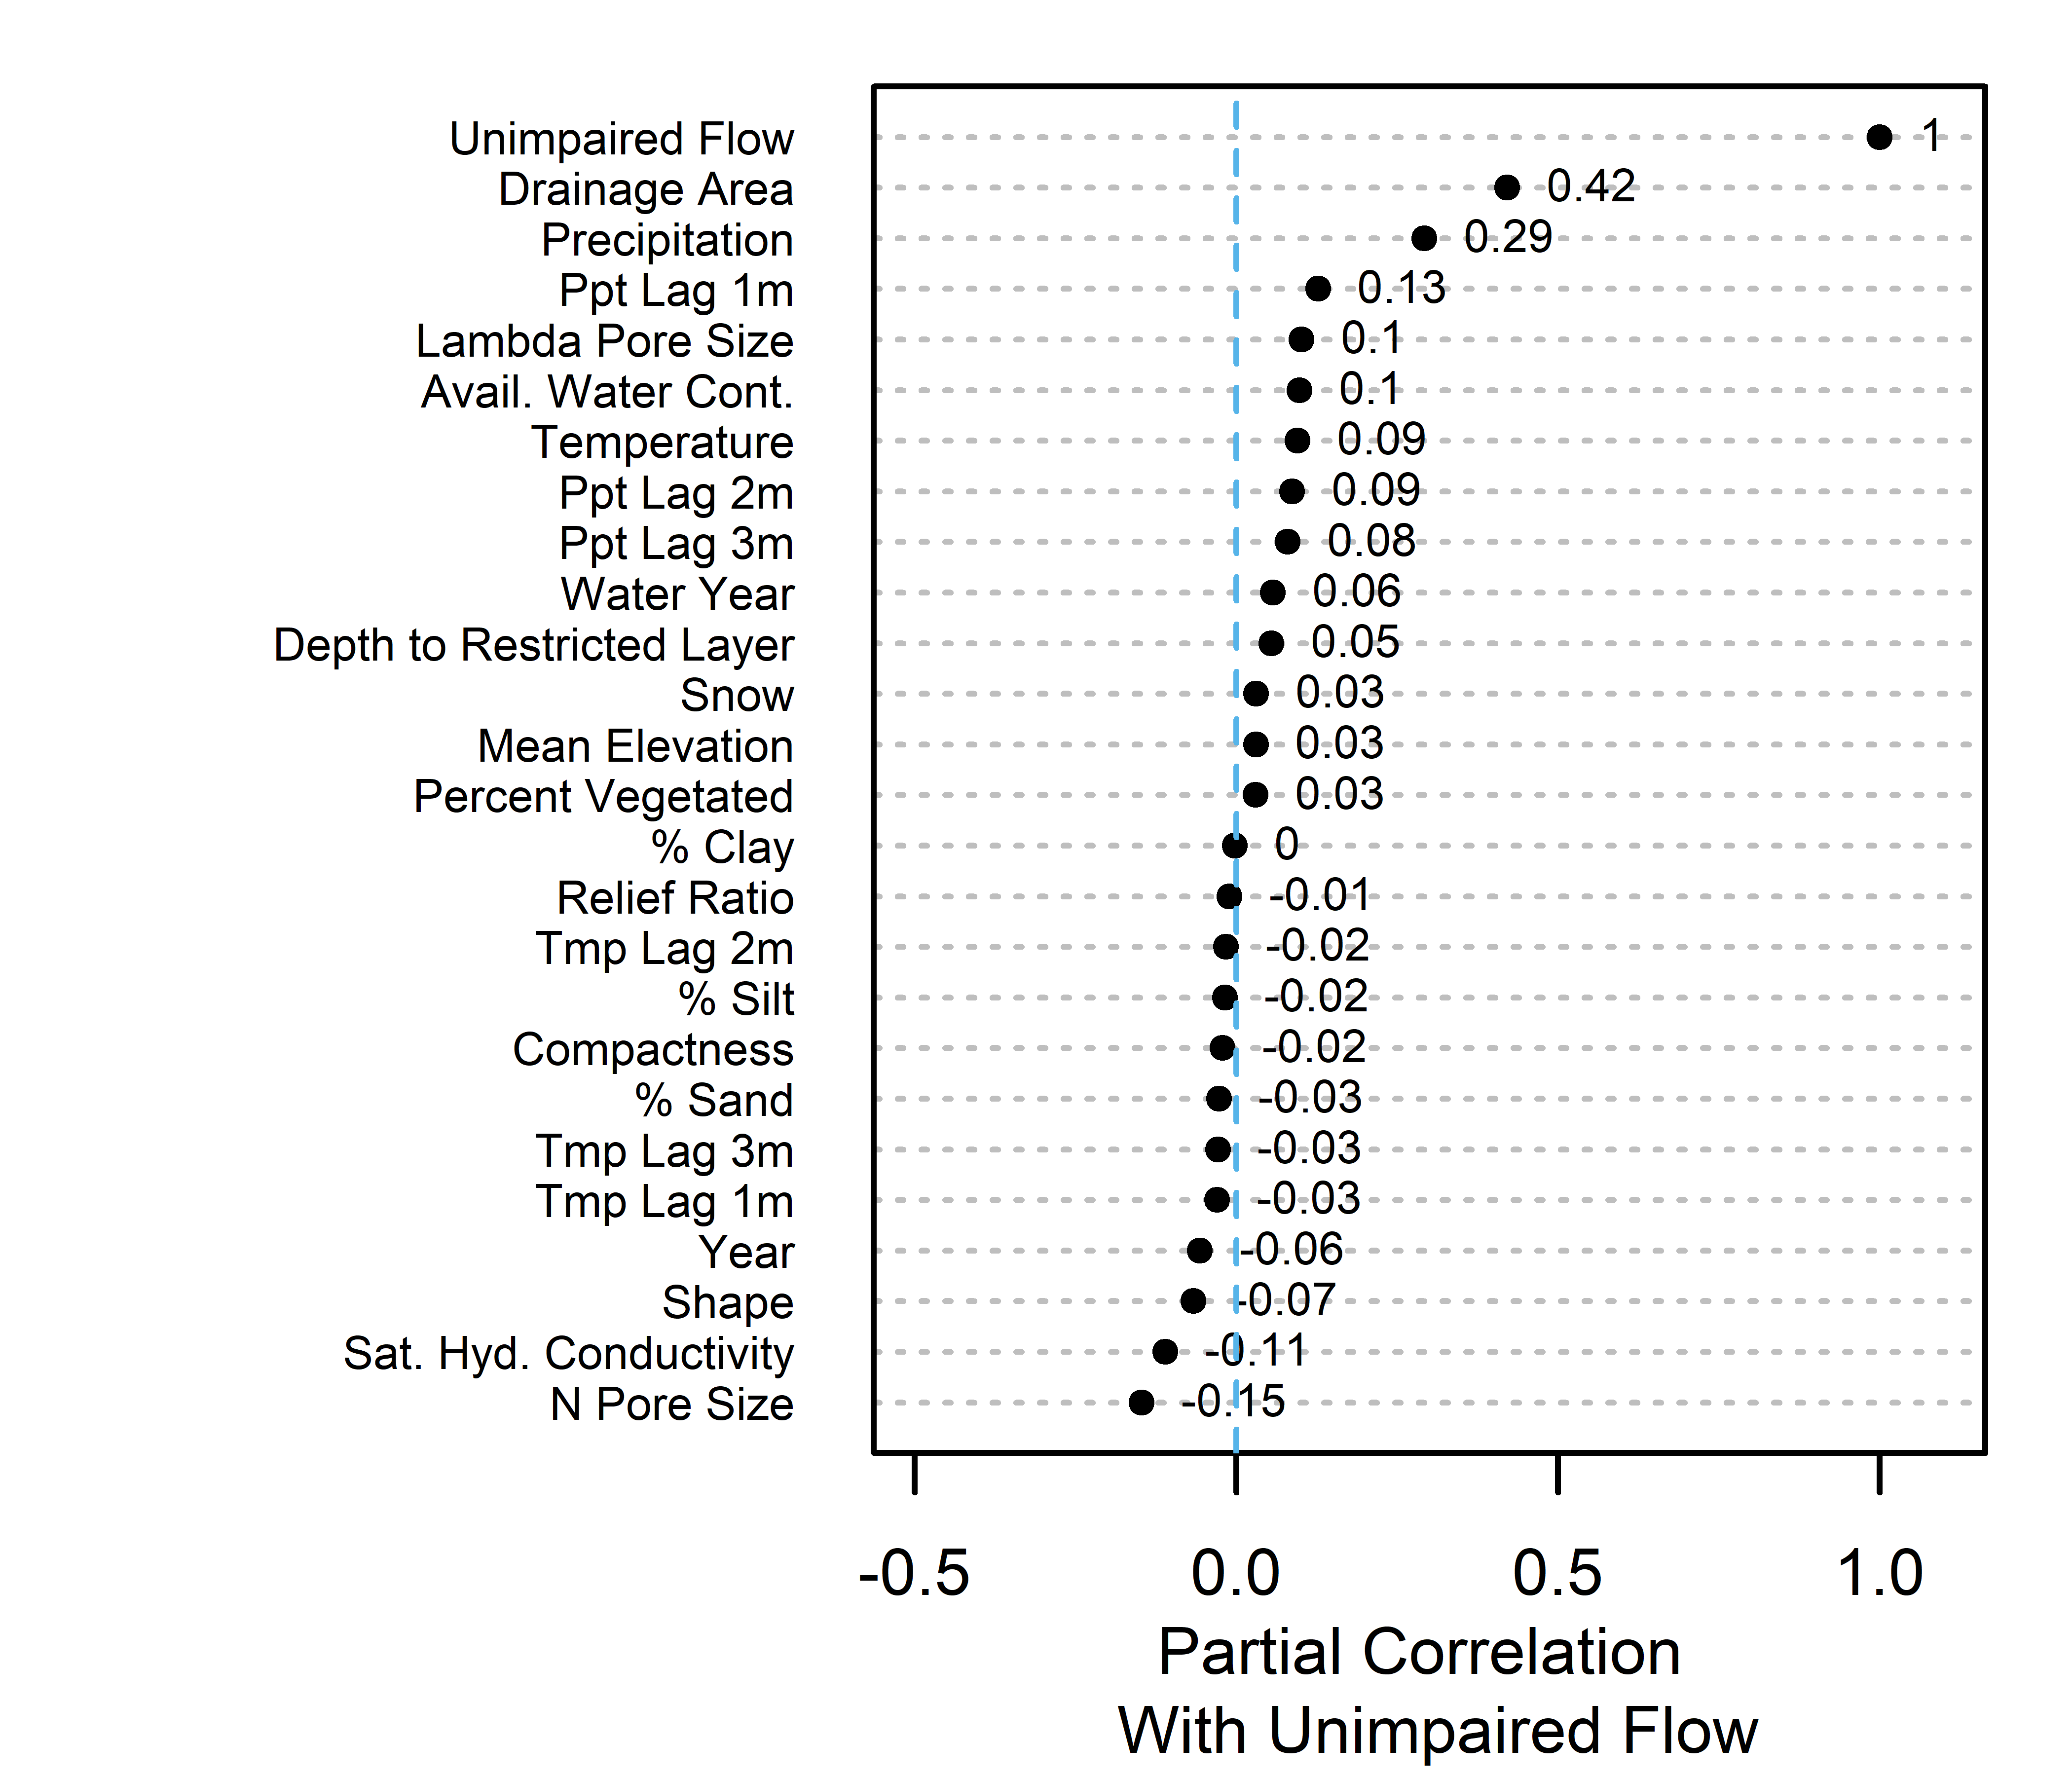
\includegraphics[width=\textwidth, trim={0 0 0 0}, clip=true]{plots/rplot08_partialcorrwithflow.png}
  		\caption{Partial Correlations}
  		\label{fig:sub2}
	\end{subfigure}
	\caption{Correlation of predictor variables with monthly flow volumes. Drainage area and precipitation correlate the most with flow.}
	\label{fig:correlogram}
\end{figure}

\begin{figure}
	\centering
	\includegraphics[width=\textwidth, trim={0 0 0 0}, clip=true]{plots/rplot07_corrplot.png}
	\caption{Correlation plot. Patterns can arise in correlations especially when some variables are calculated from or are directly related to others. For example, the percentage of sand silt and clay in a basin adds to one. Therefore, these variables are negatively correlated. Also, lag variables calculated from precipitation and temperature will tend to correlate with one another. However, the snow variable that was calculated from precipitation does not significantly correlate with precipitation.} 
	\label{fig:corrplot}
\end{figure}

